\chapter{Conducción del calor}\label{ch:b2:heat-conduction}

Tóquense un raíl metálico y un banco de madera una misma mañana fría: el
raíl se siente más frío, aunque un termómetro dé a ambos la misma
temperatura. Póngase una sartén en el fuego y su mango se calienta solo al
cabo de un rato; cávese dos metros en verano y el suelo sigue frío del
invierno; un procesador que disipa cien vatios en un centímetro cuadrado no
se funde porque encima lleva un bloque de aluminio con aletas. Todo esto es
\emph{conducción del calor}, el transporte de energía interna por la
materia gracias a la agitación de sus moléculas, sin flujo alguno de
materia --- y todo ello obedece a una ley, la de Fourier, y a una
ecuación, la del calor, que es la \omterm{thm:b2:particle-diffusion:equation}{ecuación de difusión} del capítulo
anterior con la temperatura en lugar de la densidad. Este capítulo plantea
la ley y la ecuación a partir de un balance de energía, las resuelve en los
casos que importan (paredes estacionarias y sus \omterm{prop:b2:heat-conduction:resistance}{resistencias térmicas},
calentamiento periódico y onda térmica, aletas de refrigeración), presenta
el intercambio con un fluido (ley de Newton y \omterm{def:b2:heat-conduction:biot}{número de Biot}) y calcula
la entropía que crea la conducción --- pues el calor solo fluye cuesta abajo.

\begin{omfigure}
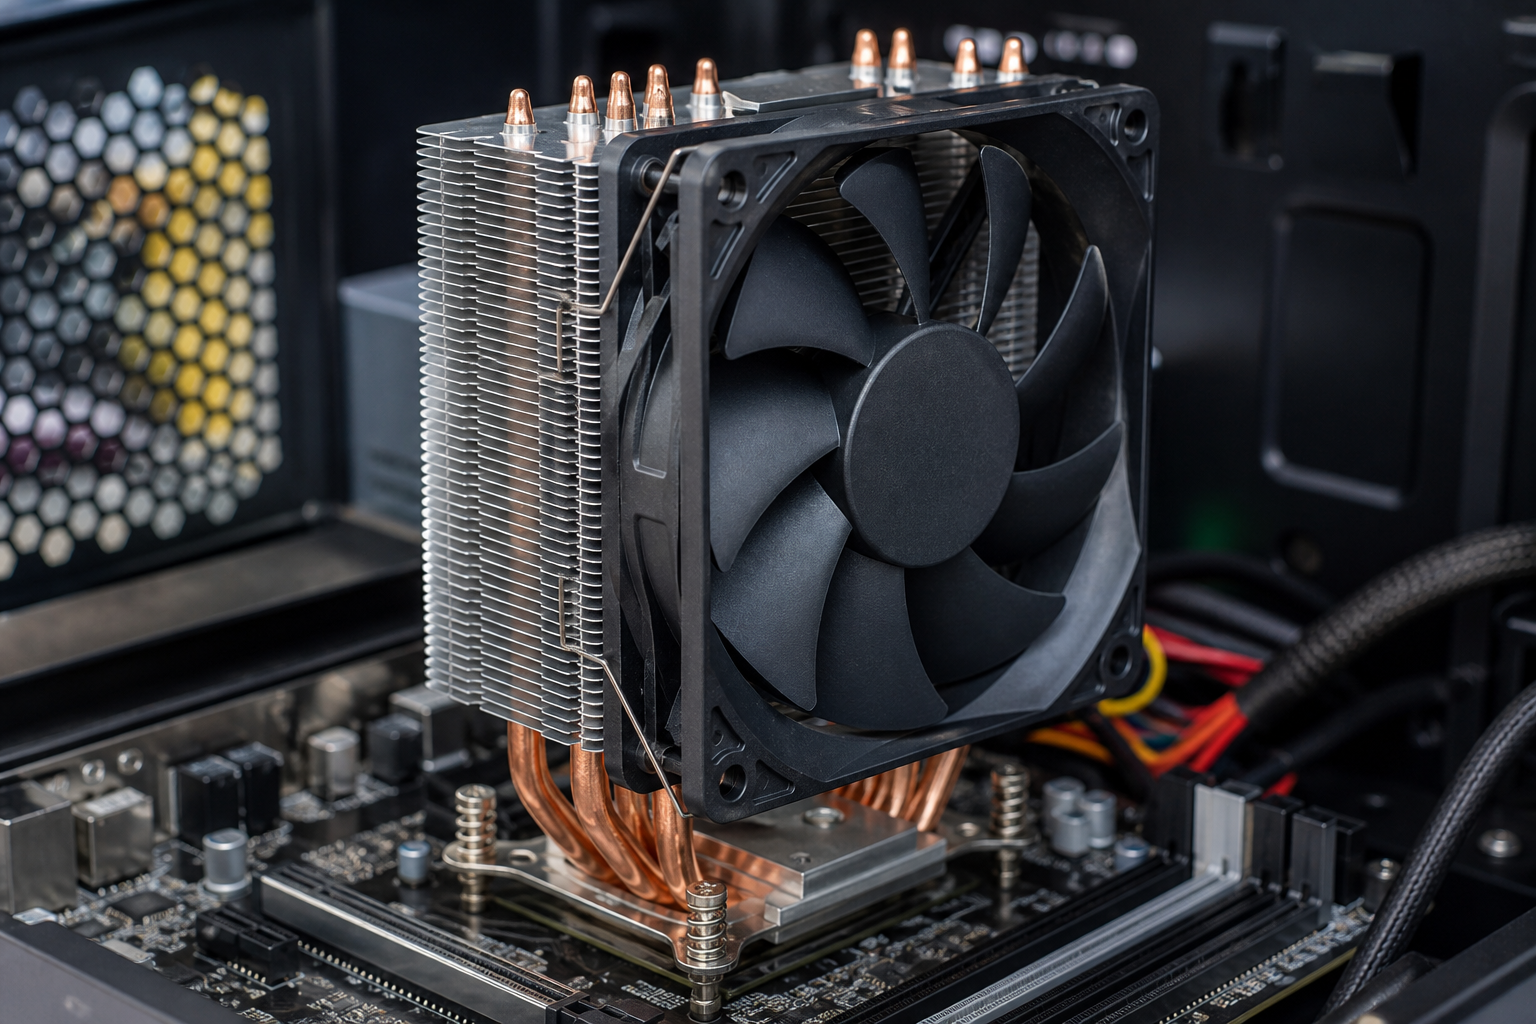
\includegraphics[width=0.58\linewidth]{images/book4/ai/b4-25-cpu-heat-sink.png}

{\small Un disipador con aletas sobre un procesador: cien vatios conducidos
fuera de un centímetro cuadrado de silicio, repartidos por una base metálica
y entregados al aire por unas aletas que multiplican por treinta la superficie.}
\end{omfigure}

\section{La ley de Fourier}

\begin{definition}[Densidad de corriente de calor]\label{def:b2:heat-conduction:flux}
La \emph{densidad de corriente de calor}\index{densidad de corriente de calor}
$\vect{j}_Q$ (en \unit{W/m^2}) es el vector tal que la energía
transferida por conducción a través de un elemento de superficie orientado
$\dd\vect S$ durante $\dd t$ vale $\vect{j}_Q\cdot\dd\vect S\,\dd t$; el
\emph{flujo térmico}\index{flujo térmico} (una potencia, en vatios) a través de una
superficie $S$ es $\Phi = \iint_S\vect{j}_Q\cdot\dd\vect S$.
\end{definition}

\begin{theorem}[Ley de Fourier]\label{thm:b2:heat-conduction:fourier}
En un medio en reposo cuya temperatura no es uniforme,
\[
\vect{j}_Q = -\lambda\,\vect{\operatorname{grad}}\,T ,
\]
donde la \emph{conductividad térmica}\index{conductividad térmica}
$\lambda > 0$ (en \unit{W/m/K}) depende del material y, débilmente, de
la temperatura. El calor fluye a favor del \omterm{def:b2:maxwell-equations:operators}{gradiente} de temperatura, de lo caliente a lo
frío --- el segundo principio incorporado a una ley lineal.
\end{theorem}

\begin{proof}
Fenomenológica, como la ley de Fick, y con la misma justificación
microscópica: las moléculas (o los electrones libres de un metal, o las
vibraciones de la red) llevan su energía en un camino aleatorio, y llega más
de ella del lado caliente.
\end{proof}

\begin{example}[Conductividades]\label{ex:b2:heat-conduction:values}
Metales (los electrones llevan el calor igual que la corriente ---
las conductividades van a la par): cobre \qty{400}{W/m/K}, aluminio
\qty{240}{W/m/K}, acero \qty{50}{W/m/K}. Sólidos aislantes: hormigón
\qty{1.5}{W/m/K}, vidrio \qty{1}{W/m/K}, ladrillo \qty{0.8}{W/m/K}, madera
\qty{0.15}{W/m/K}. Líquidos: agua \qty{0.6}{W/m/K}. Gases: aire
\qty{0.026}{W/m/K} --- y los mejores aislantes, la lana de vidrio o la espuma a
\qty{0.04}{W/m/K}, son en su mayor parte aire quieto, atrapado para que no
pueda convectar. Cuatro órdenes de magnitud del cobre al aire.
\end{example}

\section{El balance de energía y la ecuación del calor}

\begin{theorem}[Balance local de energía]\label{thm:b2:heat-conduction:balance}
En un sólido (o un fluido en reposo) de densidad $\rho$ y calor específico
$c$, con una potencia $p$ liberada por unidad de volumen (efecto Joule, una
reacción química o nuclear, radiación absorbida),
\[
\rho c\,\frac{\partial T}{\partial t} = -\operatorname{div}\vect{j}_Q + p ,
\qquad\text{en una dimensión}\quad
\rho c\,\frac{\partial T}{\partial t} = -\frac{\partial j_Q}{\partial x} + p .
\]
\end{theorem}

\begin{proof}
Primer principio para la rodaja entre $x$ y $x + \dd x$ (de sección $S$ y
volumen fijo, así que sin trabajo): su energía interna $\rho c\,T\,S\,\dd x$
cambia en $\dd t$ por el calor recibido, $[j_Q(x) - j_Q(x+\dd x)]S\,\dd t
= -\partial_x j_Q\,\dd x\,S\,\dd t$, más $p\,S\,\dd x\,\dd t$. En tres
dimensiones, el calor que entra en un volumen fijo por su superficie cerrada
vale $-\iint\vect{j}_Q\cdot\dd\vect S = -\iiint\operatorname{div}\vect{j}_Q\,\dd\tau$.
\end{proof}

\begin{theorem}[Ecuación del calor]\label{thm:b2:heat-conduction:equation}
Para $\lambda$, $\rho$ y $c$ uniformes,
\[
\frac{\partial T}{\partial t} = a\,\Delta T + \frac{p}{\rho c},
\qquad a = \frac{\lambda}{\rho c} \quad\text{(la \emph{difusividad térmica}\index{difusividad térmica}, en \unit{m^2/s})} .
\]
Vale todo lo dicho de la \omterm{thm:b2:particle-diffusion:equation}{ecuación de difusión}: linealidad,
irreversibilidad, suavizado y las escalas $L \sim \sqrt{at}$, $t \sim
L^2/a$.
\end{theorem}

\begin{proof}
Introdúzcase la ley de Fourier en el balance: $\rho c\,\partial_t T =
\lambda\Delta T + p$.
\end{proof}

\begin{example}[Difusividades y tiempos]\label{ex:b2:heat-conduction:times}
Cobre $a = \qty{1.1e-4}{m^2/s}$, aire \qty{2e-5}{m^2/s}, hormigón y
ladrillo $\approx \qty{5e-7}{m^2/s}$, agua \qty{1.4e-7}{m^2/s}, madera
\qty{1e-7}{m^2/s}. El calor cruza un centímetro de cobre en un segundo, un
centímetro de ladrillo en tres minutos, una pared de \qty{20}{cm} en un día
(por eso los muros gruesos suavizan el ciclo día--noche), el
semiespesor de \qty{1.5}{cm} de un filete en un cuarto de hora (los tiempos de
cocción escalan como el cuadrado del espesor) y un kilómetro de roca
en $10^{12}\,\unit{s}$, treinta mil años --- la Tierra sigue
enfriándose desde su formación.
\end{example}

\section{Régimen estacionario: resistencias térmicas}

\begin{proposition}[Resistencia térmica de una lámina]\label{prop:b2:heat-conduction:resistance}
En régimen estacionario y sin fuentes, una lámina de espesor $e$,
área $S$ y conductividad $\lambda$, entre las temperaturas $T_1$ y
$T_2$, tiene un perfil lineal y transporta el flujo
\[
\Phi = \frac{T_1 - T_2}{R_{\text{t}}}, \qquad
R_{\text{t}} = \frac{e}{\lambda S}\quad\text{(en \unit{K/W})} :
\]
su \emph{resistencia térmica}\index{resistencia térmica}. La temperatura
hace el papel del potencial y el flujo el de la corriente: las resistencias en
serie (capas de un muro) se suman, y las resistencias en paralelo (muro y
ventana) suman sus inversas. Para una envoltura cilíndrica (el aislamiento de una
tubería) entre los radios $r_1 < r_2$ y de longitud $\ell$,
$R_{\text{t}} = \ln(r_2/r_1)/2\pi\lambda\ell$; para una envoltura esférica,
$(1/r_1 - 1/r_2)/4\pi\lambda$.
\end{proposition}

\begin{proof}
$\dd^2T/\dd x^2 = 0$: perfil afín, $j_Q = \lambda(T_1 - T_2)/e$
uniforme, $\Phi = j_QS$. En geometría cilíndrica, $\Phi = -\lambda\,2\pi
r\ell\,\dd T/\dd r$ es el mismo para todo $r$ (sin acumulación), luego
$T = A - (\Phi/2\pi\lambda\ell)\ln r$; en geometría esférica, $\Phi =
-4\pi r^2\lambda\,\dd T/\dd r$ da $T = A + \Phi/4\pi\lambda r$.
\end{proof}

\begin{proposition}[Intercambio con un fluido: la ley de Newton]\label{prop:b2:heat-conduction:newton}
Una superficie sólida a $T_{\text{sup}}$ en contacto con un fluido a $T_{\text{fl}}$
(lejos de la superficie) pierde la densidad de flujo
\[
j_Q = h\,(T_{\text{sup}} - T_{\text{fl}}) ,
\]
donde el \emph{coeficiente de transferencia de calor}\index{coeficiente de
transferencia de calor} $h$ (en \unit{W/m^2/K}) resume la conducción a través de
la fina capa de fluido que se pega a la pared y la convección que la
renueva: $h \approx 5$--\qty{25}{W/m^2/K} para el aire en convección natural o
ligera, $50$--\qty{500}{W/m^2/K} para aire forzado y de $10^3$ a $10^4$
para el agua. La superficie añade entonces una \emph{resistencia de película} $1/hS$ en
serie con la pared.
\end{proposition}

\begin{proof}
Fenomenológica: el movimiento del fluido no se calcula, se resume
en $h$ (medido, o dado por las correlaciones de la mecánica de fluidos).
\end{proof}

\begin{omfigure}
\begin{tikzpicture}[scale=0.9, >=stealth]
  % wall layers
  \fill[omExo!15] (0,0) rectangle (1.6,2.6);
  \fill[omDef!12] (1.6,0) rectangle (2.6,2.6);
  \fill[gray!15] (2.6,0) rectangle (2.8,2.6);
  \draw (0,0) rectangle (2.8,2.6);
  \draw (1.6,0) -- (1.6,2.6); \draw (2.6,0) -- (2.6,2.6);
  \node[font=\scriptsize] at (0.8,2.85) {ladrillo};
  \node[font=\scriptsize] at (2.1,2.85) {lana};
  \node[font=\scriptsize, right] at (2.9,1.3) {interior $T_{\text{int}}$};
  \node[font=\scriptsize, left] at (-0.1,1.3) {exterior $T_{\text{ext}}$};
  \draw[->, omThm, thick] (3.6,0.7) -- (-0.8,0.7) node[midway, below, font=\scriptsize] {$\Phi$};
  % resistor chain
  \begin{scope}[yshift=-1.6cm]
    \draw (-0.8,0) -- (0.2,0);
    \draw (0.2,-0.18) rectangle (1.0,0.18); \node[font=\tiny] at (0.6,0) {$1/h_{\text{ext}}S$};
    \draw (1.0,0) -- (1.4,0);
    \draw (1.4,-0.18) rectangle (2.4,0.18); \node[font=\tiny] at (1.9,0) {$e_1/\lambda_1 S$};
    \draw (2.4,0) -- (2.8,0);
    \draw (2.8,-0.18) rectangle (3.8,0.18); \node[font=\tiny] at (3.3,0) {$e_2/\lambda_2 S$};
    \draw (3.8,0) -- (4.2,0);
    \draw (4.2,-0.18) rectangle (5.0,0.18); \node[font=\tiny] at (4.6,0) {$1/h_{\text{int}}S$};
    \draw (5.0,0) -- (5.6,0);
    \fill (-0.8,0) circle (1.5pt) node[above, font=\scriptsize] {$T_{\text{ext}}$};
    \fill (5.6,0) circle (1.5pt) node[above, font=\scriptsize] {$T_{\text{int}}$};
  \end{scope}
  % profile
  \begin{scope}[xshift=7.2cm]
    \draw[->] (0,0) -- (3.4,0) node[right, font=\scriptsize] {$x$};
    \draw[->] (0,0) -- (0,2.8) node[above, font=\scriptsize] {$T$};
    \draw[omDef, thick] (0,0.4) -- (0.3,0.6) -- (1.6,0.9) -- (2.6,2.4) -- (2.8,2.45) -- (3.2,2.6);
    \draw[dashed] (0.3,0) -- (0.3,0.6); \draw[dashed] (1.6,0) -- (1.6,0.9); \draw[dashed] (2.6,0) -- (2.6,2.4); \draw[dashed] (2.8,0) -- (2.8,2.45);
    \node[font=\scriptsize, below] at (0.95,0) {ladrillo};
    \node[font=\scriptsize, below] at (2.1,0) {lana};
    \node[font=\scriptsize, left] at (0,0.4) {$T_{\text{ext}}$};
    \node[font=\scriptsize, right] at (3.2,2.6) {$T_{\text{int}}$};
  \end{scope}
\end{tikzpicture}

{\small Un muro compuesto y su circuito térmico: película, ladrillo, lana y
película en serie. A la derecha, el perfil de temperatura --- casi toda la caída
se produce en la capa de mayor resistencia, la lana, aunque sea
la más fina.}
\end{omfigure}

\begin{example}[Un muro y una ventana]\label{ex:b2:heat-conduction:wall}
Por metro cuadrado: ladrillo de \qty{20}{cm} a \qty{0.8}{W/m/K}, $R =
\qty{0.25}{m^2.K/W}$; las dos películas, $1/8 + 1/25 = \qty{0.165}{m^2.K/W}$:
total $0.415$, es decir, $U = 1/R = \qty{2.4}{W/m^2/K}$ y, para una diferencia de
\qty{20}{K}, \qty{48}{W/m^2}. Añádanse \qty{10}{cm} de lana de vidrio, $R =
\qty{2.5}{m^2.K/W}$: el total es $2.9$, $U = \qty{0.34}{W/m^2/K}$ ---
siete veces menos. Un vidrio simple de \qty{4}{mm} a \qty{1}{W/m/K}
es todo película: $R = 0.004 + 0.165$, $U \approx \qty{6}{W/m^2/K}$; una
capa de \qty{12}{mm} de aire quieto entre dos vidrios añade $0.012/0.026 =
\qty{0.46}{m^2.K/W}$ y divide la pérdida por más de tres.
\end{example}

\begin{definition}[Número de Biot]\label{def:b2:heat-conduction:biot}
Para un sólido de tamaño $L$ que intercambia con un fluido, el \emph{número
de Biot}\index{número de Biot}
\[
\mathrm{Bi} = \frac{hL}{\lambda} = \frac{\text{resistencia interna } L/\lambda S}{\text{resistencia de película } 1/hS}
\]
compara ambas. Si $\mathrm{Bi} \ll 1$ el sólido tiene temperatura uniforme
en cada instante y se enfría como un todo, exponencialmente con
la constante de tiempo $\tau = \rho c V/hS$; si $\mathrm{Bi} \gg 1$ la
superficie está a la temperatura del fluido y el interior conduce a su
propio ritmo $L^2/a$.
\end{definition}

\section{Calentamiento periódico: la onda térmica}

\begin{proposition}[Onda térmica en un semiespacio]\label{prop:b2:heat-conduction:wave}
Si la superficie $x = 0$ de un semiespacio se mantiene a $T(0,t) = T_0 +
\theta_0\cos\omega t$, la temperatura del interior vale, en régimen
establecido,
\[
T(x,t) = T_0 + \theta_0\,\eu^{-x/\delta}\cos\Big(\omega t - \frac{x}{\delta}\Big),
\qquad \delta = \sqrt{\frac{2a}{\omega}} :
\]
una onda que se propaga hacia dentro con la celeridad $\omega\delta =
\sqrt{2a\omega}$ y se amortigua en una \emph{\omterm{def:b2:dispersion-wave-packets:complex}{profundidad de penetración}} $\delta$
por radián de fase --- en $\eu^{-2\pi} = 2 \times 10^{-3}$ por cada
longitud de onda. Las oscilaciones rápidas penetran menos que las lentas.
\end{proposition}

\begin{proof}
Búsquese $\underline T = \theta_0\eu^{\iu(\omega t - \underline k x)}$:
$\iu\omega = -a\underline k^2$, luego $\underline k^2 = -\iu\omega/a$,
$\underline k = (1 - \iu)\sqrt{\omega/2a} = (1 - \iu)/\delta$ (la raíz
que decae para $x > 0$). Tómese la parte real.
\end{proof}

\begin{omfigure}
\begin{tikzpicture}
  \begin{axis}[omaxis, width=9cm, height=4.8cm, xmin=0, xmax=4.6, ymin=-1.1, ymax=1.1,
    xlabel={$x/\delta$}, ylabel={$(T - T_0)/\theta_0$}, xtick={1,2,3,4}, ytick={-1,1}, clip=false,
    axis x line=middle, axis y line=left,
    legend style={font=\scriptsize, at={(0.98,0.04)}, anchor=south east, draw=none, fill=none}]
    \addplot[omDef, thick, domain=0:4.6, samples=120] {exp(-x)*cos(deg(-x))};
    \addlegendentry{$\omega t = 0$}
    \addplot[omThm, thick, domain=0:4.6, samples=120] {exp(-x)*cos(deg(pi/2-x))};
    \addlegendentry{$\omega t = \pi/2$}
    \addplot[omExo, thick, domain=0:4.6, samples=120] {exp(-x)*cos(deg(pi-x))};
    \addlegendentry{$\omega t = \pi$}
    \addplot[gray, dashed, domain=0:4.6, samples=60] {exp(-x)};
    \addplot[gray, dashed, domain=0:4.6, samples=60] {-exp(-x)};
  \end{axis}
\end{tikzpicture}

{\small La onda térmica en tres instantes: la oscilación de la superficie
penetra como una onda amortiguada, con la amplitud cayendo como $\eu^{-x/\delta}$
(discontinua) y la fase retrasándose en $x/\delta$ --- en $x = \pi\delta$ la
temperatura es opuesta a la de la superficie.}
\end{omfigure}

\begin{example}[El suelo, la bodega y el vino]\label{ex:b2:heat-conduction:soil}
Suelo, $a \approx \qty{5e-7}{m^2/s}$. Ciclo diario, $\omega = 2\pi/\qty{86400}{s}$:
$\delta = \qty{12}{cm}$ --- a medio metro de profundidad el día ha desaparecido. Ciclo anual:
$\delta = \qty{2.2}{m}$; a esa profundidad la oscilación de \qty{10}{K} entre verano e invierno
baja a \qty{3.7}{K} y se retrasa un radián, dos meses: la bodega es
más fría en marzo y más cálida en septiembre, y a \qty{5}{m} está a
\qty{1}{K} de ser constante --- la bodega que guarda el vino. La misma
matemática da la \omterm{def:b2:dispersion-wave-packets:complex}{profundidad de penetración} del electromagnetismo
(\cref{ch:b2:waves-in-media}): la misma ecuación, el mismo $\sqrt{2/(\text{difusividad}
\times\omega)}$.
\end{example}

\section{Aletas}

\begin{proposition}[La aleta de refrigeración]\label{prop:b2:heat-conduction:fin}
Una varilla o placa fina (de sección $S$, perímetro $p$ y conductividad $\lambda$)
sujeta en $x = 0$ a una pared a $T_0$, en un fluido a $T_{\text{fl}}$ con
el coeficiente $h$, tiene el exceso de temperatura $\theta = T - T_{\text{fl}}$
que obedece a
\[
\frac{\dd^2\theta}{\dd x^2} = m^2\theta, \qquad m = \sqrt{\frac{hp}{\lambda S}} ;
\]
para una aleta larga, $\theta = \theta_0\eu^{-mx}$ y la aleta evacúa $\Phi =
\sqrt{hp\lambda S}\,\theta_0$ --- tanto como una superficie desnuda de longitud $\sqrt{\lambda
S/hp} = 1/m$, con una temperatura que ha caído a $\theta_0/\eu$ en
$x = 1/m$. Para una aleta de longitud finita $L$ (con la punta adiabática), $\theta =
\theta_0\cosh m(L-x)/\cosh mL$ y su \emph{rendimiento}\index{rendimiento de
una aleta} --- el flujo dividido por el de una aleta isoterma a $\theta_0$ ---
vale $\eta = \tanh(mL)/mL$.
\end{proposition}

\begin{proof}
Balance estacionario de la rodaja $[x, x + \dd x]$: conducción que entra,
$-\lambda S\theta'(x)$; que sale, $-\lambda S\theta'(x + \dd x)$; perdida hacia el
fluido, $hp\,\theta\,\dd x$: $\lambda S\theta'' = hp\theta$. El flujo en la
base vale $-\lambda S\theta'(0)$: $\lambda Sm\theta_0$ para la aleta larga y
$\lambda Sm\theta_0\tanh mL$ para la finita, que hay que comparar con
$hpL\theta_0$. El \omterm{def:b2:heat-conduction:biot}{número de Biot} en el espesor de la aleta, $ht/\lambda$, debe
ser pequeño para el tratamiento unidimensional.
\end{proof}

\begin{omfigure}
\begin{tikzpicture}
  \begin{axis}[omaxis, width=6.4cm, height=4.4cm, xmin=0, xmax=3.2, ymin=0, ymax=1.12,
    xlabel={$mx$}, ylabel={$\theta/\theta_0$}, xtick={1,2,3}, ytick={1}, clip=false,
    legend style={font=\scriptsize, at={(0.98,0.98)}, anchor=north east, draw=none, fill=none}]
    \addplot[omDef, thick, domain=0:3.2, samples=60] {exp(-x)};
    \addlegendentry{aleta larga}
    \addplot[omExo, thick, domain=0:1.2, samples=60] {cosh(1.2-x)/cosh(1.2)};
    \addlegendentry{$mL = 1.2$}
    \addplot[omThm, thick, domain=0:0.5, samples=30] {cosh(0.5-x)/cosh(0.5)};
    \addlegendentry{$mL = 0.5$}
  \end{axis}
  \begin{scope}[xshift=7.2cm, yshift=0.3cm, scale=0.8, >=stealth]
    \fill[gray!25] (0,0) rectangle (0.5,3.2);
    \fill[omDef!20] (0.5,1.4) rectangle (4.2,1.8);
    \draw (0.5,1.4) rectangle (4.2,1.8);
    \node[font=\scriptsize, rotate=90] at (0.25,1.6) {pared $T_0$};
    \draw[->, omThm, thick] (0.6,1.6) -- (1.6,1.6) node[right, font=\scriptsize] {$-\lambda S\theta'$};
    \foreach \x in {1.2,2.0,2.8,3.6}{
      \draw[->, omExo] (\x,1.85) -- (\x,2.4);
      \draw[->, omExo] (\x,1.35) -- (\x,0.8);
    }
    \node[font=\scriptsize, omExo] at (2.4,2.7) {$hp\,\theta\,\dd x$};
    \node[font=\scriptsize] at (2.4,0.45) {fluido $T_{\text{fl}}$};
  \end{scope}
\end{tikzpicture}

{\small A la izquierda, la temperatura a lo largo de una aleta, para una aleta larga y dos
finitas (de punta adiabática) --- más allá de $mx \approx 2$ una aleta aporta poco. A la derecha,
el balance de una rodaja: conducción a lo largo y convección hacia fuera por el
perímetro.}
\end{omfigure}

\begin{example}[Un disipador]\label{ex:b2:heat-conduction:sink}
Aletas de aluminio de \qty{1}{mm} de espesor ($p/S \approx 2/t = \qty{2000}{m^{-1}}$)
y \qty{30}{mm} de alto, en aire forzado con $h = \qty{50}{W/m^2/K}$: $m =
\sqrt{2h/\lambda t} = \qty{20}{m^{-1}}$, $mL = 0.6$, $\eta = 0.89$ --- las
aletas trabajan al $89\%$ de su área. Treinta de ellas, de \qty{60}{mm} de ancho,
ofrecen \qty{0.11}{m^2} donde el cuadrado desnudo de \qty{60}{mm} ofrecía
\qty{0.0036}{m^2}: una resistencia $1/\eta hA = \qty{0.2}{K/W}$ en vez de
\qty{5.6}{K/W}; \qty{100}{W} elevan la base \qty{20}{K} en vez de
\qty{560}{K}. Alargar las aletas gana poco (la $\tanh$ satura) y afinarlas
pierde rendimiento: $mL \approx 1$ es el compromiso del ingeniero.
\end{example}

\section{Entropía creada por la conducción}

\begin{proposition}[Producción de entropía]\label{prop:b2:heat-conduction:entropy}
Un flujo $\Phi$ conducido de un cuerpo a $T_{\text{cal}}$ a un cuerpo a
$T_{\text{fr}} < T_{\text{cal}}$ a través de una pared estacionaria crea entropía con
el ritmo
\[
\dot S_{\text{c}} = \Phi\Big(\frac{1}{T_{\text{fr}}} - \frac{1}{T_{\text{cal}}}\Big) > 0 ;
\]
localmente, la conducción crea $\sigma_s = \lambda\,(\vect{\operatorname{grad}}\,T)^2/T^2
\ge 0$ por unidad de volumen y tiempo --- nula solo donde la temperatura es
uniforme. La conducción del calor es irreversible: la misma energía, entregada a
temperatura menor, puede hacer menos trabajo.
\end{proposition}

\begin{proof}
El estado de la pared no cambia, así que su entropía es constante: el cuerpo
caliente pierde $\Phi/T_{\text{cal}}$ por unidad de tiempo y el frío gana
$\Phi/T_{\text{fr}}$; la diferencia se crea. Localmente, el balance de entropía
$\partial_t(\rho s) + \operatorname{div}(\vect{j}_Q/T) = \sigma_s$
con $\rho T\partial_t s = -\operatorname{div}\vect{j}_Q$ da $\sigma_s =
\vect{j}_Q\cdot\vect{\operatorname{grad}}(1/T) = -\vect{j}_Q\cdot
\vect{\operatorname{grad}}\,T/T^2 = \lambda(\vect{\operatorname{grad}}\,T)^2/T^2$.
\end{proof}

\begin{method}[Estimaciones de conducción]\label{meth:b2:heat-conduction:method}
(1) Estacionario: constrúyase el circuito térmico --- láminas $e/\lambda S$, películas
$1/hS$, envolturas $\ln(r_2/r_1)/2\pi\lambda\ell$; en serie y en paralelo.
(2) Transitorio: $\mathrm{Bi} = hL/\lambda$; si es pequeño, $\tau = \rho cV/hS$; si es
grande, $t \sim L^2/a$. (3) Periódico: $\delta = \sqrt{2a/\omega}$, amortiguamiento
$\eu^{-x/\delta}$, retraso $x/\delta$. (4) Fuentes: $p$ por unidad de volumen, perfiles
parabólicos. (5) Aletas: $m = \sqrt{hp/\lambda S}$, $\eta = \tanh(mL)/mL$. (6)
Entropía: $\Phi(1/T_{\text{fr}} - 1/T_{\text{cal}})$.
\end{method}

\section{Ejercicios}

\begin{exercise}[$\star$]\label{exo:b2:heat-conduction:1}
Un muro de ladrillo de \qty{20}{cm} de espesor ($\lambda = \qty{0.8}{W/m/K}$) y \qty{100}{m^2},
entre \qty{20}{\celsius} dentro y \qty{0}{\celsius} fuera
(con las superficies a esas temperaturas): densidad de flujo, flujo total; y con
\qty{10}{cm} de lana de vidrio (\qty{0.04}{W/m/K}) añadidos.
\end{exercise}

\begin{exercise}[$\star$]\label{exo:b2:heat-conduction:2}
Difusividades: cobre ($\lambda = 400$, $\rho = 8900$, $c = \qty{385}{J/kg/K}$),
hormigón ($1.5$, $2300$, $900$) y madera ($0.15$, $600$, $2500$). Tiempos que tarda el calor
en cruzar \qty{1}{cm} y \qty{20}{cm} de cada uno; y los \qty{30}{km} de corteza de
la Tierra.
\end{exercise}

\begin{exercise}[$\star$]\label{exo:b2:heat-conduction:3}
Vidrio simple (\qty{4}{mm}, $\lambda = \qty{1}{W/m/K}$) con películas $h_{\text{int}}
= 8$, $h_{\text{ext}} = \qty{25}{W/m^2/K}$; vidrio doble con una capa de \qty{12}{mm}
de aire quieto (\qty{0.026}{W/m/K}): valores de $U$ y flujos para
\qty{20}{K}. ¿Por qué es el vidrio doble real casi el doble de malo que esta
estimación, y qué hacen el argón y los tratamientos de baja emisividad?
\end{exercise}

\begin{exercise}[$\star$]\label{exo:b2:heat-conduction:4}
Cocina: $a = \qty{1.4e-7}{m^2/s}$ para la carne. Tiempo que tarda el centro de un
filete de \qty{3}{cm} en notar la sartén; y el de un asado de \qty{12}{cm}. Un pavo
del doble de peso: ¿cuánto más tarda (la dimensión escala como la raíz cúbica
de la masa)?
\end{exercise}

\begin{exercise}[$\star\star$]\label{exo:b2:heat-conduction:5}
\emph{Fuente interna.} Un cilindro de radio $R$ libera $p$ por unidad de
volumen; la superficie está a $T_{\text{sup}}$. (a) Muéstrese que $T(r) = T_{\text{sup}} +
p(R^2 - r^2)/4\lambda$. (b) Hilo de cobre, $R = \qty{1}{mm}$, $j =
\qty{1e7}{A/m^2}$, $\gamma = \qty{6e7}{S/m}$: $p$ y la diferencia entre centro y
superficie. (c) Barra de combustible nuclear, $R = \qty{5}{mm}$, $p = \qty{3e8}{W/m^3}$,
$\lambda = \qty{3}{W/m/K}$: la misma pregunta. (d) Coméntese.
\end{exercise}

\begin{exercise}[$\star\star$]\label{exo:b2:heat-conduction:6}
\emph{El suelo.} (a) Dedúzcase $\delta = \sqrt{2a/\omega}$. (b) Suelo con
$a = \qty{5e-7}{m^2/s}$: \omterm{def:b2:dispersion-wave-packets:complex}{profundidades de penetración} diaria y anual. (c) Profundidad
a la que la amplitud anual es la décima parte de la de la superficie; retraso de fase
allí. (d) Una tubería de agua no debe helarse donde la temperatura invernal de la superficie
baja a \qty{-10}{\celsius} en torno a una media de
\qty{10}{\celsius}: profundidad mínima (onda anual).
\end{exercise}

\begin{exercise}[$\star\star$]\label{exo:b2:heat-conduction:7}
\emph{Biot.} (a) Esfera de cobre de \qty{1}{cm} de radio, en aire ($h =
\qty{10}{W/m^2/K}$): \omterm{def:b2:heat-conduction:biot}{número de Biot} y constante de tiempo de su enfriamiento. (b) Una
patata ($\lambda = \qty{0.5}{W/m/K}$, $a = \qty{1.4e-7}{m^2/s}$, radio
\qty{3}{cm}) en un horno con $h = \qty{20}{W/m^2/K}$: \omterm{def:b2:heat-conduction:biot}{número de Biot}; ¿qué
tiempo gobierna su cocción? (c) ¿Por qué se hace pequeña la punta de un termopar?
(d) ¿Por qué se enfría más deprisa una taza de café si se remueve o se sopla ---
qué resistencia cambia?
\end{exercise}

\begin{exercise}[$\star\star$]\label{exo:b2:heat-conduction:8}
\emph{Una aleta.} (a) Dedúzcanse $\theta'' = m^2\theta$ y la solución de la aleta larga.
(b) Aleta de aluminio de \qty{1}{mm} de espesor y \qty{30}{mm} de alto, en convección
natural con $h = \qty{20}{W/m^2/K}$: $m$, $mL$ y rendimiento. (c) ¿En qué
factor multiplica la aleta el área de intercambio de su huella, y
el flujo? (d) ¿Por qué es un desperdicio de metal una aleta muy larga o muy fina?
\end{exercise}

\begin{exercise}[$\star\star$]\label{exo:b2:heat-conduction:9}
\emph{Tuberías.} (a) Dedúzcase la resistencia de una envoltura cilíndrica. (b) Una
tubería de vapor, de radio exterior \qty{5}{cm} a \qty{150}{\celsius}, envuelta en
\qty{5}{cm} de lana de vidrio, con aire a \qty{20}{\celsius} y $h =
\qty{10}{W/m^2/K}$ fuera: pérdida por metro, comparada con la tubería desnuda.
(c) Muéstrese que la resistencia total del aislamiento más la película tiene un
mínimo en el \emph{radio crítico} $r_{\text{cr}} = \lambda/h$. (d) Para un
hilo eléctrico de \qty{1}{mm} de radio con una funda de plástico ($\lambda =
\qty{0.2}{W/m/K}$), ¿enfría o calienta la funda al cobre?
\end{exercise}

\begin{exercise}[$\star\star\star$]\label{exo:b2:heat-conduction:10}
\emph{Entropía.} El muro de \cref{exo:b2:heat-conduction:1} (desnudo)
entre \qty{293}{K} y \qty{273}{K}. (a) Entropía creada por segundo.
(b) Calcúlese $\int\sigma_s\,\dd V$ con el perfil lineal y compruébese que
coincide. (c) Entropía creada una vez aislado. (d) El trabajo que una
máquina reversible podría haber extraído de los \qty{8}{kW} entre
esas temperaturas, y qué queda de él tras el muro.
\end{exercise}

\begin{exercise}[$\star\star\star$]\label{exo:b2:heat-conduction:11}
\emph{Por qué el metal se siente frío.} (a) Para la onda térmica, calcúlese el
flujo en la superficie $j_Q(0,t)$ y muéstrese que adelanta a la temperatura de la superficie en
$\pi/4$, con la amplitud $\sqrt{\lambda\rho c\,\omega}\,\theta_0$. La
magnitud $b = \sqrt{\lambda\rho c}$ es la \emph{efusividad}. (b) Dos
semiespacios a $T_1$ y $T_2$ se ponen en contacto: admitiendo que
cada uno sigue entonces un perfil de erfc con la temperatura común de la superficie
$T_{\text{cont}}$, y escribiendo la continuidad del flujo en el contacto,
muéstrese que $T_{\text{cont}} = (b_1T_1 + b_2T_2)/(b_1 + b_2)$. (c) Piel
($b \approx \qty{1000}{J/m^2/K/s^{1/2}}$, \qty{33}{\celsius}) que toca
cobre ($b = 37000$) o madera ($b = 400$) a \qty{20}{\celsius}: temperaturas
de contacto. (d) ¿Por qué se siente más frío un suelo de baldosa que una alfombra a
la misma temperatura, y por qué es solo transitoria la sensación?
\end{exercise}

\begin{exercise}[$\star\star\star$]\label{exo:b2:heat-conduction:12}
\emph{Enfriar una lámina.} Una lámina $-L < x < L$ a $T_0$ se sumerge en $t =
0$ en un baño a $T_{\text{fl}}$ con $h \to \infty$. (a) Muéstrese que $\theta =
T - T_{\text{fl}}$ admite las soluciones $\cos(k_nx)\,\eu^{-ak_n^2t}$ con $k_n
= (2n+1)\pi/2L$. (b) Desarróllese la condición inicial en serie de Fourier
sobre esos modos y escríbase la solución completa. (c) Tras los primeros
instantes, ¿qué modo sobrevive y cuál es la constante de tiempo? (d) Tiempo
que tarda el centro de un filete de \qty{3}{cm} ($a = \qty{1.4e-7}{m^2/s}$) en quedar
dentro del $1\%$ del baño.
\end{exercise}

\section{Problema: aislar una casa, refrigerar un procesador}

\begin{problem}[{Problema de fin de semana --- la conducción a la escala de un
edificio y de un chip}]\label{pb:b2:heat-conduction:1}
Datos: ladrillo $\lambda = \qty{0.8}{W/m/K}$, $\rho = \qty{1800}{kg/m^3}$, $c =
\qty{840}{J/kg/K}$; lana de vidrio \qty{0.04}{W/m/K}; vidrio \qty{1}{W/m/K}; aire
quieto \qty{0.026}{W/m/K}; aluminio \qty{240}{W/m/K}, $\rho = \qty{2700}{kg/m^3}$,
$c = \qty{900}{J/kg/K}$; silicio \qty{150}{W/m/K}; pasta térmica
\qty{5}{W/m/K}; suelo $a = \qty{5e-7}{m^2/s}$, $\lambda = \qty{1}{W/m/K}$;
películas $h_{\text{int}} = 8$, $h_{\text{ext}} = \qty{25}{W/m^2/K}$.

\textbf{Parte I --- La casa.}
Una casa tiene \qty{100}{m^2} de muros (ladrillo de \qty{20}{cm}) y \qty{20}{m^2}
de ventanas de vidrio simple (\qty{4}{mm}); dentro \qty{20}{\celsius} y
fuera \qty{0}{\celsius}.
\begin{enumerate}
  \item Resistencia por metro cuadrado del ladrillo solo; densidad de flujo
        si sus caras estuvieran a las dos temperaturas.
  \item Con las dos películas: $R$ y $U = 1/R$ por metro cuadrado; lo mismo
        con \qty{10}{cm} de lana de vidrio añadidos.
  \item $U$ del vidrio simple; y de un vidrio doble con \qty{12}{mm}
        de aire quieto.
  \item Pérdida total de la casa antes y después de aislar los muros
        y doblar las ventanas.
  \item En una temporada de calefacción de $2500$ grados-día (la integral de
        la diferencia de temperatura a lo largo de la temporada, en \unit{K.d}),
        energía perdida antes y después, en kilovatios hora.
  \item Temperatura de la superficie interior del muro, desnudo y aislado;
        ¿por qué resulta incómodo un muro frío y le sale moho?
  \item Tiempo de difusión a través del ladrillo; ¿qué le hace al
        ciclo día--noche?
\end{enumerate}

\textbf{Parte II --- El suelo bajo la casa.}
\begin{enumerate}[resume]
  \item Dedúzcase la \omterm{def:b2:dispersion-wave-packets:complex}{profundidad de penetración} $\delta = \sqrt{2a/\omega}$ de una
        onda térmica.
  \item $\delta$ diaria y anual en el suelo.
  \item Profundidad a la que la oscilación diaria baja al $1\%$; amplitud
        anual a \qty{2.2}{m} y a \qty{5}{m} para una oscilación superficial de \qty{10}{K}.
  \item Retraso de fase a \qty{2.2}{m}, en días: ¿cuándo está más fría la bodega?
  \item Flujo de calor en la superficie de la onda anual (amplitud y fase);
        compárese su amplitud con el flujo geotérmico de \qty{0.06}{W/m^2}.
  \item El \omterm{def:b2:maxwell-equations:operators}{gradiente} geotérmico es de \qty{30}{K/km}: compruébese con el
        flujo y $\lambda$, y explíquese por qué es invisible en las
        estaciones de la bodega.
\end{enumerate}

\textbf{Parte III --- El procesador.}
Un chip disipa \qty{100}{W} en una pastilla de \qty{1}{cm^2} y \qty{0.5}{mm}
de espesor; una capa de \qty{50}{\micro m} de pasta sobre \qty{10}{cm^2} lo une
a un disipador de aluminio: base de \qty{60}{mm} $\times$ \qty{60}{mm} $\times$
\qty{5}{mm}, con treinta aletas de \qty{60}{mm} de ancho, \qty{30}{mm} de alto y \qty{1}{mm}
de espesor; un ventilador da $h = \qty{50}{W/m^2/K}$; ambiente a \qty{25}{\celsius}.
\begin{enumerate}[resume]
  \item Densidad de flujo a través de la pastilla; resistencia de la pastilla.
  \item Resistencia de la pasta; y si la sustituyera un hueco de aire de \qty{50}{\micro m}.
  \item Parámetro de aleta $m$, $mL$ y rendimiento; compruébese el \omterm{def:b2:heat-conduction:biot}{número de Biot}
        en el espesor de la aleta.
  \item Área total de las aletas y resistencia de las aletas; resistencia de
        la base (conducción por \qty{5}{mm}); temperatura de unión.
  \item Lo mismo sin aletas (cuadrado desnudo de \qty{60}{mm}): conclusión.
  \item El ventilador se para ($h = \qty{10}{W/m^2/K}$): temperatura de unión;
        ¿qué hace el procesador a \qty{100}{\celsius}?
  \item Masa y capacidad calorífica del disipador; su constante de tiempo $RC$;
        y la de la pastilla sola (\qty{0.1}{g}, \qty{700}{J/kg/K}).
  \item ¿Por qué tienen los buenos disipadores una base de cobre o caloductos?
\end{enumerate}

\textbf{Parte IV --- La entropía.}
\begin{enumerate}[resume]
  \item Entropía creada por segundo por la envolvente desnuda de la casa
        (pregunta 4) entre \qty{293}{K} y \qty{273}{K}; y tras
        el aislamiento.
  \item Entropía creada por los \qty{100}{W} del chip al pasar de la
        unión al ambiente; y por la conversión de trabajo eléctrico
        en calor en la pastilla.
  \item Muéstrese que para una lámina $\int\sigma_s\,\dd V = \Phi(1/T_{\text{fr}} -
        1/T_{\text{cal}})$.
  \item Resúmase en cinco líneas qué gobierna un muro, una aleta, una bodega
        y un chip.
\end{enumerate}
\end{problem}
